\def\CTeXPreproc{Created by ctex v0.2.9, don't edit!}
%\documentclass{beamer}
\documentclass[%handout,
xcolor=pdftex]{beamer}
\mode<presentation> {
  \usetheme{Warsaw}
  \setbeamercovered{transparent}
}
\let\Tiny=\tiny
\usetheme{Singapore}
\usecolortheme{dolphin}
\usepackage{amsmath}
\usepackage{textcomp}
\usepackage{amssymb}
\usepackage{amsthm}
\usepackage{graphicx}
\usepackage{color}
\usepackage{lipsum}
\usepackage{hyperref}
\usepackage{multirow}
\usepackage{bm}
\DeclareMathSymbol{\Phi}{\mathalpha}{operators}{8}
%\setbeamertemplate{headline}{}
\setbeamertemplate{footline}[page number]
\newcommand\Fontvi{\fontsize{9pt}{8}\selectfont}
\newcommand\Fontvii{\fontsize{7pt}{8}\selectfont}
\newcommand{\backupbegin}{
   \newcounter{finalframe}
   \setcounter{finalframe}{\value{framenumber}}
}
\newcommand{\backupend}{
   \setcounter{framenumber}{\value{finalframe}}
}\newtheorem{proposition}{Proposition}
\title{Unit 22: Linear Filters}
\author[STAT 5170: Applied Time Series, Unit 24]{Jeffrey Woo}
\institute{Department of Statistics, University of Virginia}
\date{Spring 2020}

\AtBeginSubsection[] {
  \begin{frame}<beamer>{Outline}
    \tableofcontents[currentsection,currentsubsection]
  \end{frame}
}



\begin{document}


\frame{\titlepage}


\begin{frame}
\frametitle{Readings for Unit 22}

Textbook chapter 4.7 (until page 214).

\end{frame}


\begin{frame}
\frametitle{Last Unit}
\begin{enumerate}
\item Smoothing periodogram to reduce variance.
\end{enumerate}
\end{frame}

\begin{frame}
\frametitle{Motivation}

Some of the previous topics have suggested that one could ``transform" a time series to modify the distribution of its spectral density or variance. In this unit we will define a linear filter and show how it can be used to extract signals from a time series.


\end{frame}

\section{Linear Filter}
\frame{\tableofcontents[currentsection]}

\begin{frame}
\frametitle{Linear Filter}

The linear filter modifies the spectral characteristics of a time series in a predictable way. Let  $x_t,t=0,\pm 1,\pm 2,\ldots,$ be a stationary \textbf{input
series}, and $a_j,j=0,\pm 1,\pm 2,\ldots,$ be a set of specified
coefficients. We use the linear filter $\{a_j,j=0,\pm 1, \pm
2,\ldots\}$ to operate on $\{x_t,t=0,\pm 1, \pm 2,\ldots\}$ to
produce an \textbf{output series}
\begin{eqnarray}\label{eq:1}
y_t = \sum^\infty_{j=-\infty} a_j x_{t-j}.
\end{eqnarray}



\end{frame}

\begin{frame}
\frametitle{Linear Filter}

(\ref{eq:1}) is sometimes called a convolution.  $y_t$ is a linear combination of $x_t$'s, suggesting the
name ``linear filter''. The coefficients $a_r$ are collectively
called the \underline{\hspace{45 mm}}.

\end{frame}

\begin{frame}
\frametitle{Linear Filter}

\textbf{Example}: Recall that a causal ARMA model
$\phi(B)y_t =\theta(B)w_t$ has the causal representation
$y_t=\sum^\infty_{j=0}\psi_j w_{t-j}$. This is a special case
of (\ref{eq:1}) with $a_j=0$ for $j<0$. 

\begin{itemize}

\item $y_t$ in
(\ref{eq:1}) depends on all $x$'s (both past and future)
whereas causal ARMA model depends only on past values. 

\item In (\ref{eq:1}), we do NOT assume that $x_t$ is a white noise
series. Instead $x_t$ can be any stationary series.

\end{itemize}

\end{frame}

\begin{frame}
\frametitle{Linear Filter}

Let $\gamma_x(h)=E[(x_{t+h}-Ex_{t+h})(x_t-Ex_t)]$ denote the
autocovariance function of $x_t$, and the spectral density is denoted by
\begin{eqnarray*}
 f_x(\omega) = \sum^\infty_{h=-\infty} \gamma_x(h)e^{-2\pi \omega i h}.
 \end{eqnarray*}
The inverse Fourier transform formula is
\begin{eqnarray*}
 \gamma_x(h) = \int^{0.5}_{-0.5} f_x(\omega) e^{2\pi \omega i h} d\omega.
 \end{eqnarray*}

\end{frame}

\begin{frame}
\frametitle{Linear Filter}

\begin{eqnarray} \label{eq:3}
\gamma_y(h) &=& \hspace{50mm} \nonumber \\
            &=& \hspace{50mm} \nonumber \\
            &=& \hspace{50mm} \nonumber \\
            &=& \hspace{50mm} \nonumber \\
            &=& \hspace{50mm} \nonumber \\
            &=& \hspace{50mm} \nonumber \\
            &=& \hspace{50mm} \nonumber \\
            &=& \hspace{50mm}
\end{eqnarray}

\end{frame}

\begin{frame}
\frametitle{Linear Filter}

Note that
\begin{eqnarray} \label{eq:res}
A_{yx}(\omega) = \sum^\infty_{j=-\infty} a_j e^{-2\pi \omega i j}
\end{eqnarray}
is the Fourier transform of $a_j$ and called the \underline{\hspace{35 mm}} function. We require $\sum^\infty_{j=-\infty}|a_j|<\infty$ to ensure that
$A_{yx}(\omega)$ is well defined.

\end{frame}

\begin{frame}
\frametitle{Linear Filter}

Now we compute the spectral density $f_y(\omega)$ of $y_t$. By
the inverse Fourier transform,
\begin{eqnarray}\label{eq:4}
\gamma_y(h)  = \int^{0.5}_{-0.5} f_y(\omega) e^{2\pi \omega i h}d\omega.
\end{eqnarray}
Comparing (\ref{eq:4}) and (\ref{eq:3}), we find that
\begin{eqnarray}\label{eq:5}
f_y(\omega)  =  \hspace{50mm}.
\end{eqnarray}


\end{frame}

\begin{frame}
\frametitle{Linear Filter}

We can use (\ref{eq:5}) to compute the exact effect on the spectrum of any given filtering operation. The spectrum of the input series is changed by filtering and the effect of the change is characterized as a frequency-by-frequency multiplication by the squared magnitude of the frequency response function, $A_{yx}(\omega)$. $|A_{yx}(\omega)|^2$ is called the \underline{\hspace{25 mm}} function.

\end{frame}

\begin{frame}
\frametitle{Linear Filter}

Suppose two filtering operations are applied to a stationary series $x_t$ in succession, e.g.:

$$
y_t = \sum_{j=-\infty}^{\infty} a_j x_{t-j},
$$

and then

$$
z_t = \sum_{k=-\infty}^{\infty} b_k y_{t-k}.
$$

The spectrum of the output is

$$
f_z(\omega) = |A(\omega)|^2 |B(\omega)|^2 f_x(\omega).
$$

\end{frame}

\section{Worked Examples I}
\frame{\tableofcontents[currentsection]}

\begin{frame}
\frametitle{Worked Example: MA(1)}

\textbf{Question}: Consider an MA(1) process $y_t = w_t + \theta w_{t-1}$. Given that $f_w(\omega) = \sigma_w^2$, derive the spectral density of this MA(1) process using (\ref{eq:5}).

\vspace{50mm}

\end{frame}

\begin{frame}
\frametitle{Worked Example: AR(1)}

\textbf{Question}: Consider an AR(1) process $y_t = 0.5 y_{t-1} + w_{t}$. Given that $f_w(\omega) = \sigma_w^2$, derive the spectral density of this AR(1) process using (\ref{eq:5}).

\vspace{50mm}

\end{frame}

\begin{frame}
\frametitle{Worked Example: First Difference Filter}

\textbf{Question}: Consider the first difference filter $y_t = \nabla x_t = x_t - x_{t-1}$. Derive the power transfer function for this filter and comment on the practical implications.

\vspace{50mm}

\end{frame}

\begin{frame}
\frametitle{Worked Example: First Difference Filter}

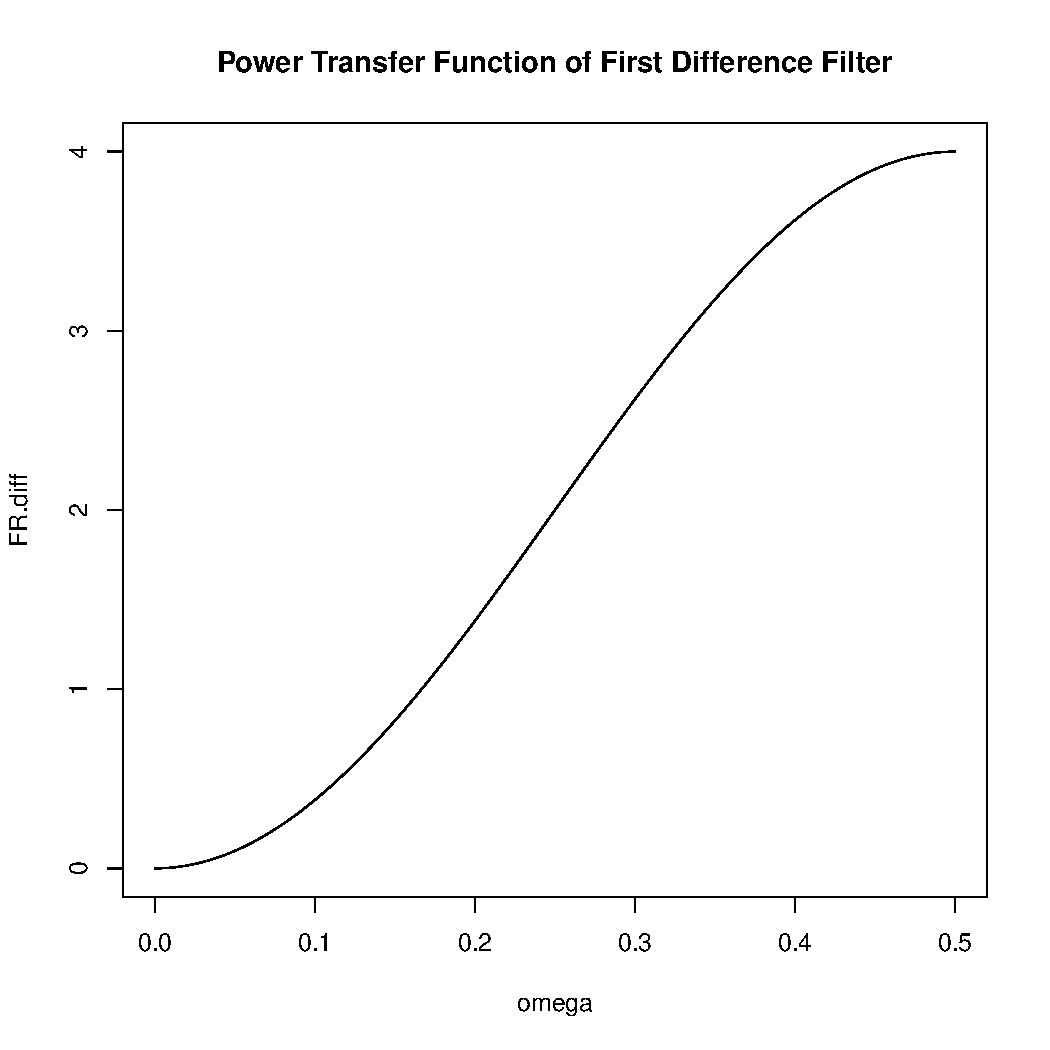
\includegraphics[width=110mm, height=75mm]{diff.pdf}

\end{frame}

\begin{frame}
\frametitle{Worked Example: Moving Average Filter}

\textbf{Question}: Consider the following moving average filter $y_t = \frac{1}{24} (x_{t-6} + x_{t+6}) + \frac{1}{12}\sum_{j=-5}^5 x_{t-j}$. Derive the power transfer function for this filter and comment on the practical implications.

\vspace{50mm}

\end{frame}

\begin{frame}
\frametitle{Worked Example: Moving Average Filter}

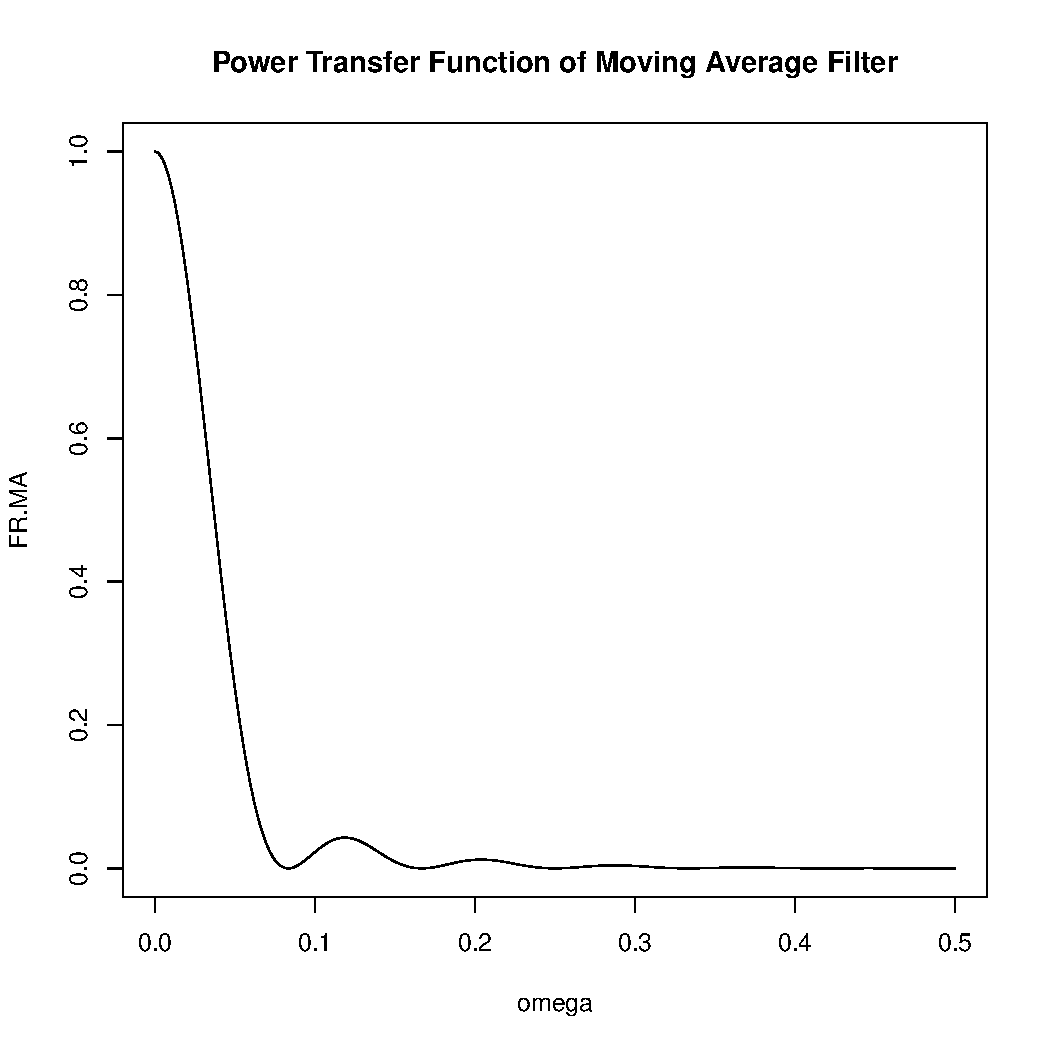
\includegraphics[width=110mm, height=75mm]{ma.pdf}

\end{frame}

\section{Worked Examples II}
\frame{\tableofcontents[currentsection]}

\begin{frame}
\frametitle{Worked Example: SOI Dataset}

We'll apply the first difference and 12-month moving average filters to the SOI dataset.

\end{frame}

\begin{frame}
\frametitle{Worked Example: SOI Dataset}

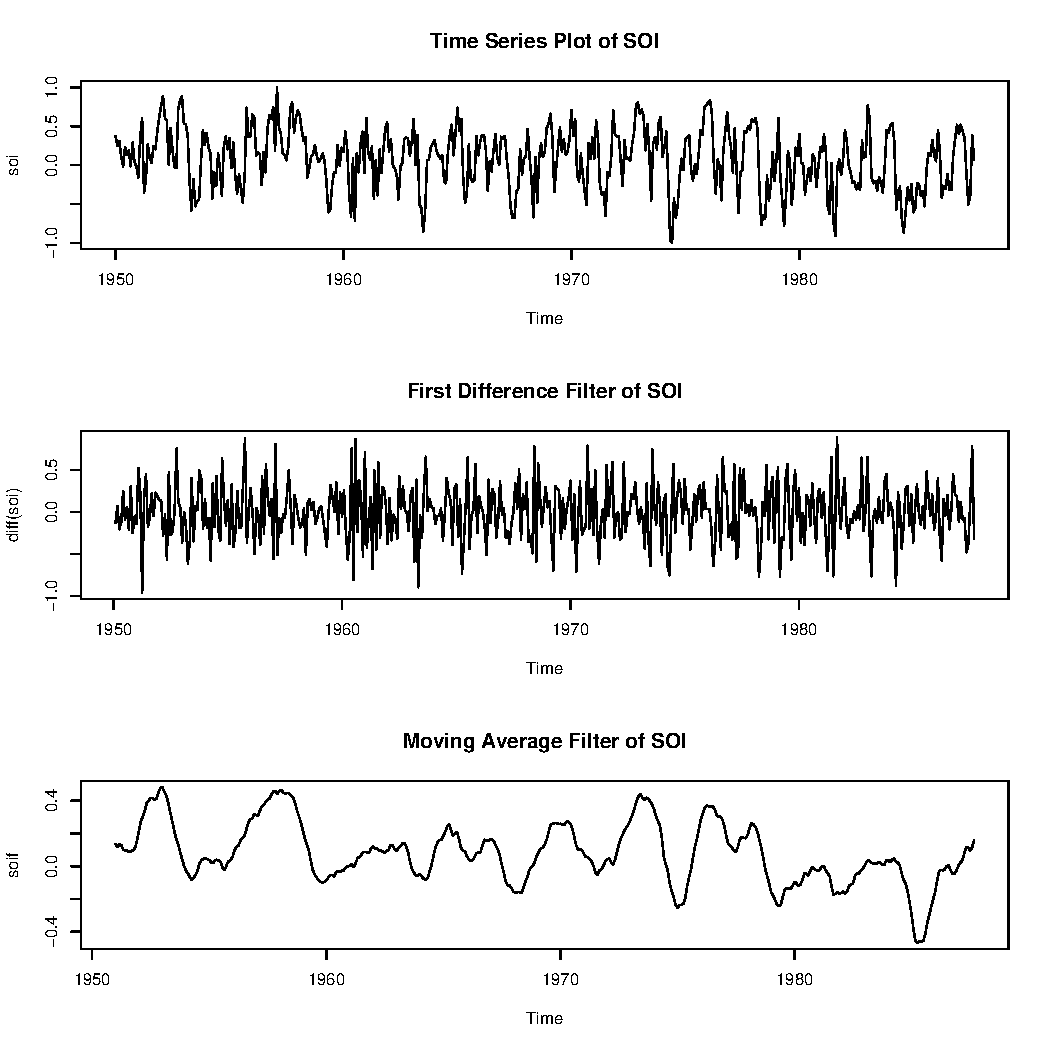
\includegraphics[width=110mm, height=75mm]{ts.pdf}

\end{frame}


\begin{frame}
\frametitle{Worked Example: SOI Dataset}

\begin{itemize}
\item The first difference filter retained the higher frequencies.
\item The moving average filter retained the lower frequencies. Enhances the component associated with El Ni$\tilde{\text{n}}$o and dampens the seasonal/yearly component.
\end{itemize}

\end{frame}

\begin{frame}
\frametitle{Worked Example: SOI Dataset}

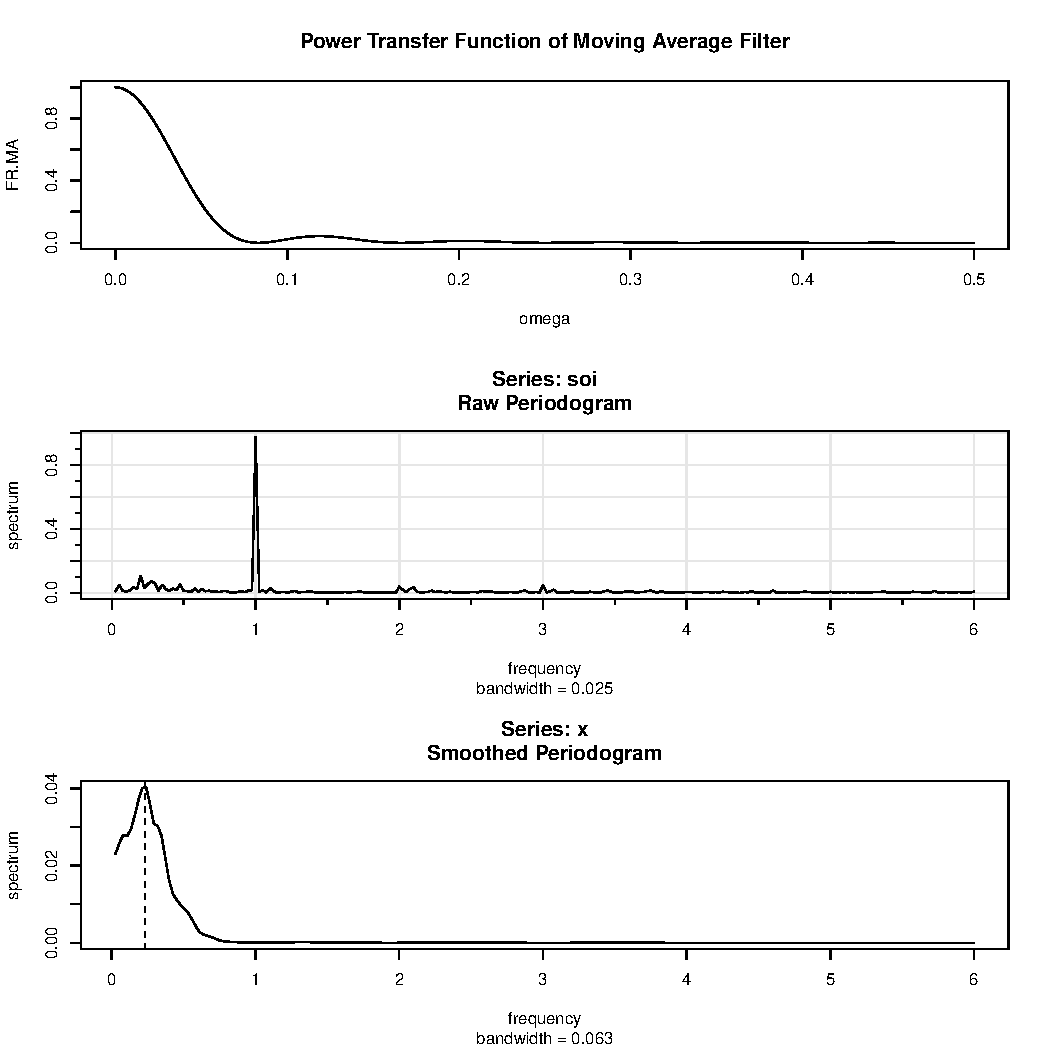
\includegraphics[width=110mm, height=75mm]{raw.pdf}

\end{frame}



\begin{frame}
\frametitle{Worked Example: SOI Dataset}

From the periodogram of the moving average filtering of the data, high frequency behavior has been removed. El Ni$\tilde{\text{n}}$o frequency around $1/52$. 

\end{frame}





\begin{frame}
\frametitle{Worked Example: SOI Dataset}

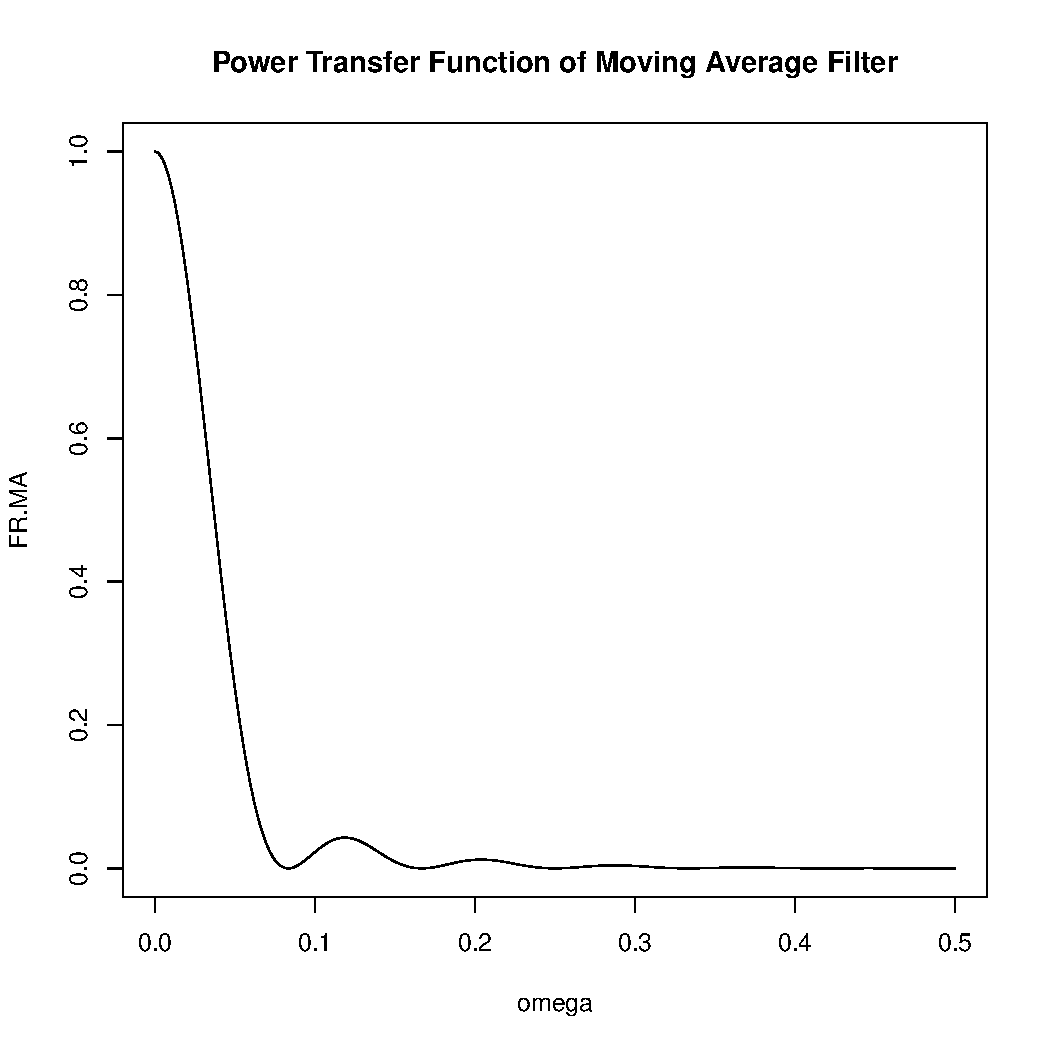
\includegraphics[width=110mm, height=55mm]{ma.pdf}

For the 12-month moving average filter, frequencies higher than around 0.08 will be ``cut off". Periods shorter than $1/0.08 = 12.5$ months will be dampened, and the El Ni$\tilde{\text{n}}$o frequency is retained.

\end{frame}

\end{document} 